\section{Research}
\subsection{Blockchain}

%\subsection{Blockchain}
%% TODO Technical knowledge needed to implement
%% TODO How it works?
%% TODO Why use it?
%
%\subsection{Existing solutions}
%
%\subsubsection{Copyright law}
%% TODO The state of the current copyright system
%\subsubsection{Online rights management}
%% TODO How do creators manage protection of their work
%
%\subsection{Development theory}
%% TODO Explanation of agile development methodology
%% TODO TDD and Scrum
%
%\subsection{Aims of the solution}
% TODO The over arcing aims of the solution, aka what should the system fix

The theory of a \keyword{blockchain} is not new \cite{origins_blockchain} but the implementation and hype around \keyword{blockchains} is new and extremely popular in the current day thanks to Bitcoin designed by Satoshi Nakamoto based on their white paper \cite{nakamoto2008bitcoin}. The accepted benefits of a \keyword{blockchain} are decentralisation, distribution, and immutability.For a \keyword{blockchain} to exist and be useful it needs nodes to maintain the data structure authenticate all transactions and hash the current block in preparation for the next in the chain.

\begin{figure}[H]
\caption{Blockchain structure with transactions saved in Merkle trees\cite{btc-white}}
\centering
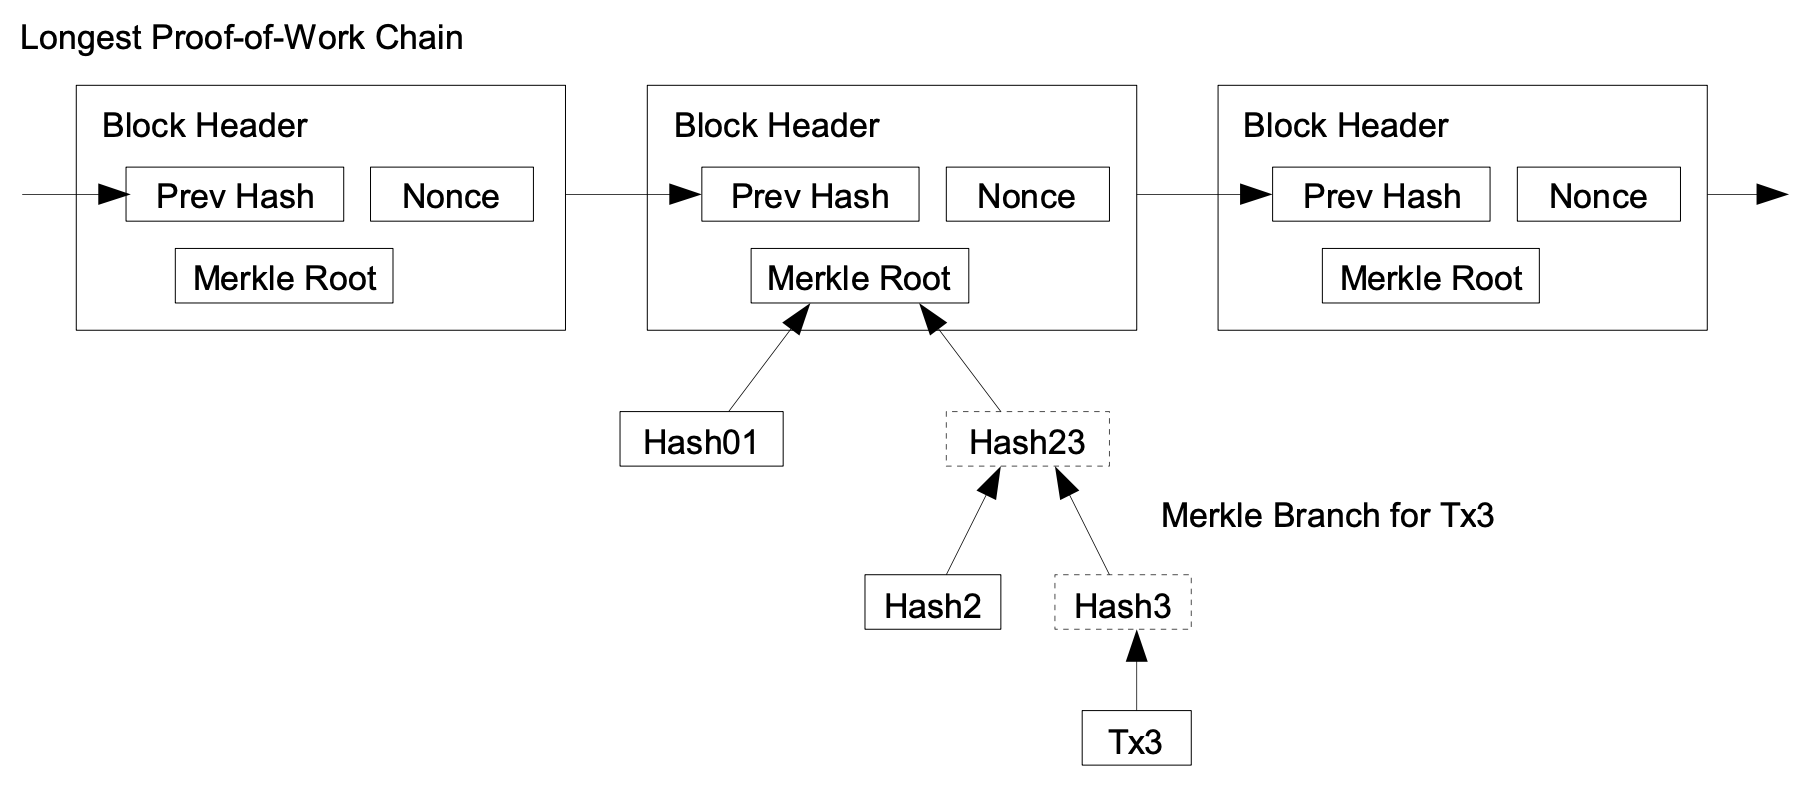
\includegraphics[width=\textwidth,height=0.4\textheight,keepaspectratio]{images/patterns/merkle}
\centering
\end{figure}

\subsubsection{Technical proficiencies / limitations}

{\noindent\regular\textbf{Proficiencies}\vspace{2mm}}

\begin{description}
	\item[Security] Is the core of \keyword{blockchain} as the cryptographic hashing strategy is what makes the data structure a chain.
	\item[Transparency] Is not intrinsic to \keyword{blockchains} that is down to the implementation (public or private), however the underlying concept facilitates and promotes this open and transparent behaviour simply by the fact that nodes within a \keyword{blockchain} network need a copy of all transactions/blocks.
	\item[Decentralisation] Is definitely the most popular benefit of \keyword{blockchains} and it's not a technical benefit just like transparency decentralisation is a social debate that is made possible by technical decisions of the \keyword{blockchain} architecture, centred around the control and ownership of peoples data \begin{quote}"It avoids concentrations of power that could let a single person or organization take control."\cite{bohme2015bitcoin}\end{quote} 
\end{description}

{\noindent\regular\textbf{Limitations}\vspace{2mm}}

\noindent\keyword{Blockchain} technology faces two major limitations, the largest chains in the world (Bitcoin and \keyword{Ethereum}) are quickly growing in size which has pointed out scaleability problems caused by transaction speed and cost per transaction which are currently slow and expensive respectively compared to traditional systems (cost experiments have borne this out in the aptly named paper "Comparing blockchain and cloud services for business process execution"\cite{rimba2017comparing} and show that business logic on \keyword{blockchains} are 2 orders of magnitude more expensive than current cloud services).

\keyword{Blockchains} rely on \keyword{consensus protocols} which is a mathematical formula to determine consensus of the network, essentially enough of the nodes have to agree the current state of the \keyword{blockchain} whenever it's modified. Currently all major chains including Bitcoin and \keyword{Ethereum} use a protocol called proof of work\cite{PoW} which uses the total amount of compute a node has produced as the comparable proof that can be verified by many other nodes easily. This has worked so far for these major chains however ballooning energy consumption (which can be seen in realtime at the \href{https://ccaf.io/cbeci/index}{Cambridge Bitcoin Electricity Consumption Index}), high transaction costs, and inadequate transaction processing bandwidth is forcing them to change and look for solutions.

\keyword{Ethereum} have decided to completely reinvent their consensus protocol with a fundamentally different protocol called proof of stake which promises reduced energy consumption, cheaper, and faster transactions\cite{PoS}. Although there have been other proposed solutions including: improving the proof of stake system by parallelising it across nodes\cite{fi12080125} or reducing the block size for a increase transaction capacity by reducing the amount of work needed per block with a security trade off to balance\cite{kiayias2015speed}.

\subsubsection{Use of blockchain for IP protection}

I am not the first person to have thought of representing and enforcing \keyword{copyright} protection on a distributed \keyword{blockchain}, there has actually been a lot of discussion around the topic showing the benefits of using this technology for \keyword{copyright} such as transparency; \begin{quote} "Blockchain may substantially increase visibility and availability of information about copyright ownership." \cite{Copyright_in_the_blockchain_era} \end{quote} the power of \keyword{smart contracts} and utilising a networks cryptocurrency \begin{quote} "Smart contracts will allow automatic and instantaneous payments to designated parties, and expiration of a license after a certain amount of time." \cite{Copyright_in_the_blockchain_era} \end{quote} and simplification through the globalisation of \keyword{copyright} law. majority opinion says that introducing \keyword{smart contracts} to \keyword{blockchain} technology is extremely powerful particularly within \keyword{copyright} law to \begin{quote}"reliably automate a large volume of ‘dumb transactions’" \cite{missing_link_in_copyright_licensing}\end{quote} which will greatly reduce friction by removing unnecessary work and removing expertise needed currently in the field to be properly protected.

\subsubsection{Use of blockchain for legal purposes}

Bringing \keyword{copyright} to \keyword{blockchain} is apart of a larger conversation about the compatibility of any legal or even governmental workflows to be either represented or completely reinvented using \keyword{blockchain} technology, and it does look like in many cases these types of problems can leverage \keyword{blockchain} and possibly even thrive.

The legal industry is notoriously complicated requiring a great level of knowledge and expertise in the field to make sense of anything or more importantly get anything done. Logically laws make an obvious starting point for computerisation because computers are defined systems of ridged laws however this didn't make sense during the first wave of \keyword{blockchains} which almost entirely focused its efforts towards currency. The introduction of \keyword{smart contracts} has opened up the possibilities for automated law processing massively reducing boilerplate and bulky legal work which is largely trivial but time consuming.

\begin{quote}
	"So-called ‘smart contracts’ built on blockchain technologies may prove to be the most important example yet of “self-executing, customised rules”." \cite{MILLARD2018843}
\end{quote}

For governing \keyword{blockchains} ledger and transparency will take centre stage as essentially all governments are big collections of "things", assets, people and information. Not only are they collections but historical records, thankfully \keyword{blockchains} are immutable, timestamped, secure and built for openness. Because \keyword{blockchains} are just general purpose data structures there're uses are broad; \begin{quote}"keeping an overview of the authorities provided in a public organization and the ability to change the authority only if there is agreement among nodes which are classified as being higher ranked in the hierarchy." \cite{OLNES2017355}\end{quote}

% TODO Probably not needed, bit of a rehash of other sections

%\subsection{Copyright law}
%
%What is the reason for "fixing" \keyword{copyright}? is it broken? \keyword{Copyright} law is old, it was first introduced from the 1700s to the 1800s with the introduction of the printing press and the first true \keyword{copyright} act being the Statute of Anne in 1710 which has morphed into the Copyright, Designs and Patents Act 1988 in the UK (\href{https://www.legislation.gov.uk/ukpga/1988/48/contents}{see}) and the Copyright Act of 1976 in the US. The fact that each country has its own unique \keyword{copyright} laws (even though the international Berne Convention exists local jurisdictions still apply) exacerbated by the internet has been showing signs of cracks especially when "digital goods" are involved.
%
%Theses issues can be broken down into three key areas: 
%
%\begin{enumerate}
%	\item \textbf{Legal transparency/complexity} Is the absolutely at the top of this list, as a creative can you be sure your work is protected in every jurisdiction possible? No you can't because the current copyrighting system is a sparse disconnected collection of closed databases. Implementing a globally open database of copyrighted works with consistent rules and digital finger printing. 
%	\item \textbf{Royalty distributions (compensation)} Monetary transactions are the current forte of all major \keyword{blockchains} so why not simplify one of the hardest tasks for an creator, receiving payment for the use of a work of course this has become easier with the introduction of internet payments and purpose built systems like "PRS for Music" but integrating royalty payments straight into the \keyword{copyright} registration proves for secure and cohesive system.
%	\item \textbf{Cost} Of protection a work is essentially free as the Berne Convention prohibits the registration of a work as a requirement to protection (\keyword{copyright} is born with the work), however legally protecting and defending authorship of a work is not free and can be devastating not to mention extremely one sided (massive record company vs band). With the help of an immutable global ledger determining who registered the work is simple.
%\end{enumerate}
%
%These problems and solutions in this section are talked about in the paper \textit{Copyright in the blockchain era: Promises and challenges} \cite{Copyright_in_the_blockchain_era}

%\section{Environment and crypto} not enough for this section

\subsection{The market}

The vast majority of \keyword{blockchain} applications in the current day are financial for obvious reasons with the market capitalisation of cryptocurrencies being the universal metric for the \keyword{blockchain} markets size \cite{wood_2021}, however the health care industry has been aggressively investigating and implementing \keyword{blockchain} technology particularly in the secure distribution of medical data and health records \cite{8167115}, supply chain technology has seen some innovation tracking goods as they pass through a chain. 